\chapter{Discussion}
\label{chap:results}

After strictly presenting results in the last chapter, this one will discuss the results, more specifically, their implications and possible reasons. 
The sequence of results to be discussed remains the same as before.


\section{MVTecAD LOCO Experiments}
\label{sec:locoresultssota}

When comparing the detection and localization results of the approaches analyzed in the last chapter, quality significantly drops. 
Although the average in most cases is out of context still an acceptable result, it poses a poor performance compared with the prior 
IAD standards. Where on the MVTecAD \cite{MVTEC_Bergmann_2021} most approaches were strictly in a high-performance interval above 98 percent 
instance classification and above 97 percent for anomaly localization, a drop of from 10 up to 30 percent in some classes is drastic and significant. 
Combined with inferences from Fig. \ref{fig:structvslogic}, this information strongly suggests that the latest state-of-the-art anomaly detection approaches are not inherently practical when detecting logical anomalies. The poor sPRO results also support this. GCAD \cite{LOCODentsAndScratchesBergmann2022}, the approach uniting global and local representations introduced in its 
paper, demonstrates an average sPRO of $0.701$ over all classes, which is significantly above the approaches analyzed here. This last argument is most important because this metric 
is an effective way to observe segmentation capabilities. \newline
Another aspect to consider is the nature of both datasets. The MVTecAD \cite{MVTEC_Bergmann_2021} generally uses smaller images than the 
logical dataset and more straightforward motives. As the IAD approaches generally shrink input images through resizing for efficiency reasons, 
potentially helpful information, as well as necessary one when dealing with small anomalies, may be lost. 
Moreover, as visible in Fig. \ref{fig:mvtecexampleimages} and Fig. \ref{fig:pushpinviz}, the MVTecAD LOCO dataset 
has many more objects and motives in one image than merely a simple texture or tile. This makes for much more complex images and anomalous objects 
to detect and thus represents an increased level of complexity over the other dataset. This may also emphasize the performance 
difference between analyzed approaches and methods reviewed in \cite{LOCODentsAndScratchesBergmann2022}. \newline
According to Bergmann et al. \cite{LOCODentsAndScratchesBergmann2022}, the main challenges of the logical dataset are tiny regions, logical constraints that are 
not bound to a specific region, and anomalies in confusing regions with a texture that is hard to differentiate (Fig. \ref{fig:difficultAnomalies}). This was also observable in the results.

\begin{figure}[htbp]
    \centering
    \begin{subfigure}[b]{\textwidth}
        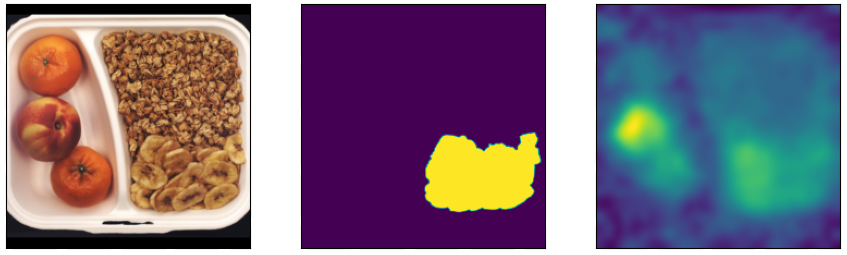
\includegraphics[width=0.45\textwidth]{figures/difficultAnomalies/breakfast_box_test_logical_anomalies_011.png}
        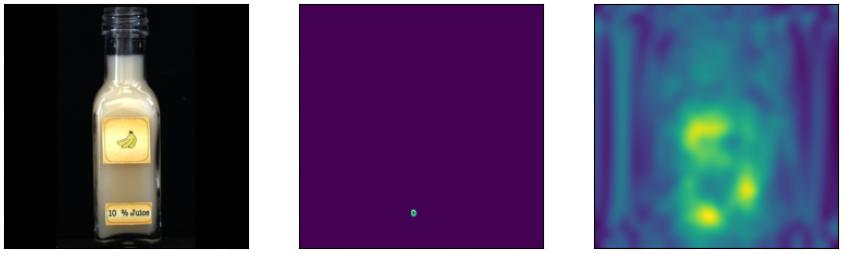
\includegraphics[width=0.45\textwidth]{figures/difficultAnomalies/juice_bottle_test_structural_anomalies_059.png}

    \end{subfigure}
    \begin{subfigure}[b]{\textwidth}
        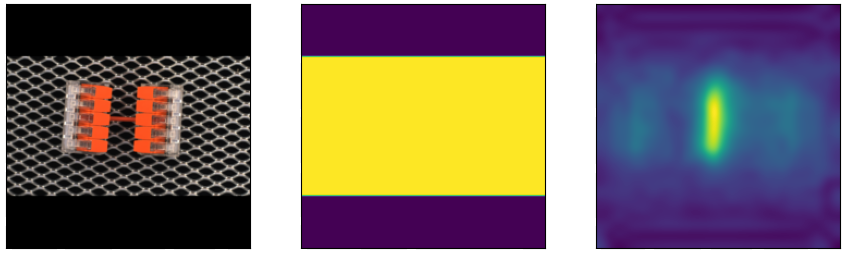
\includegraphics[width=0.45\textwidth]{figures/difficultAnomalies/splicing_connectors_test_logical_anomalies_064.png}
        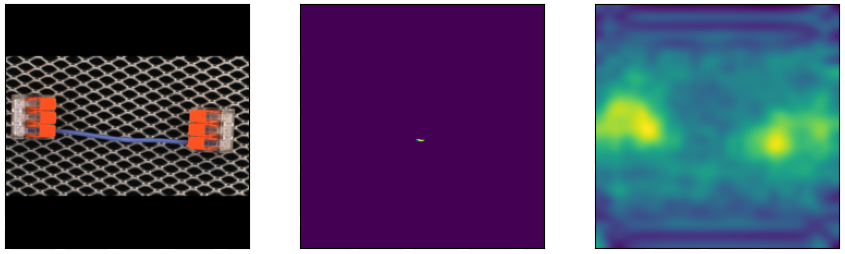
\includegraphics[width=0.45\textwidth]{figures/difficultAnomalies/splicing_connectors_test_structural_anomalies_001.png}

    \end{subfigure}
    \caption{MVTecAD LOCO \cite{LOCODentsAndScratchesBergmann2022} anomalies with lots of texture and very small anomalous regions.}
    \label{fig:difficultAnomalies}
\end{figure}


\section{Flat Connector}
\label{sec:flatconnectordiscussion}

The performance of previous IAD approaches on the novel dataset class is displayed in section \ref{sec:faltconnectorxperiments}. The performance here generally was higher 
than in other logical anomaly classes. Picking up on named difficulty discrepancies from the last section, the results combined with the nature of the flat connector images 
are consistent with other results. The object in this class possesses a smooth surface, sharp edges, and no accessories. With these 
characteristics, it is different from classes like the breakfast box or screw bag, which possess either random textures or unique properties 
like the semitransparency of the plastic bag. On the other hand, the class also consists of logical anomalies that potentially look 
like structural ones. An example of this would be the extra hole, which has the same structural properties as other small holes and is 
just misplaced. The flat connector class is thus technically a complementary class of the logical dataset but comprises 
one of the easier classes in that set. \newline
As expected, the structural anomaly segmentations were much more precise overall than logical ones. Among logical anomalies, 
missing holes were localized most precisely. This leads one to conclude that the methods used to fake such an anomaly were not applied perfectly. 
Visual artifacts that are visible after such preprocessing of the class objects were unavoidable with the existing resources and  
helped to detect the anomalies. The logical anomalies that posed the toughest challenge for most classifiers regarding localization 
were the extra hole and the differently sized one. \newline
Structural anomalies yielded a generally good segmentation if the classifier displayed overall sufficient performance. Cut-off edges were straightforward to localize, which is also to be expected since they very noticeably break the object's contour. Broken edges provided for 
varying performance depending on the classifier. Scratches mainly were detected correctly, although the segmentations were often 
thicker than the anomalous region.



\section{Ensemble Performance}
\label{sec:ensemblediscussion}

Ensembles in IAD are not a focus of current research. Some papers \cite{patchCore2022} provide homogeneous ensembles as a complementary option. 
PatchCores ensemble is simple average voting, meaning multiple classifier instances are trained and evaluated on the same inputs. The outputs are then averaged on an image and pixel level. 
This may lead to a slight performance improvement, as in this example. 
With our approach, however, we aimed at transcending minor improvements, utilizing feature-level ensemble strategies to achieve even more robust anomaly localization performance.
The ensemble experiments conducted in this work did not yield an increased performance, as seen in chapter \ref{chap:experiments}. 
Possible reasons for the shortcomings of each experiment are discussed in the following subsections.

\subsection{Independent Transformation Block}
\label{subsec:ITBfaildiscussion}

During the experiments chapter \ref{chap:experiments}, it was observable that the independent transformation block \cite{EnsembleHeller2023} did not produce any usable results. 
Since this method is reported to function as intended in Heller et al., there has to be some circumstance that is the root of the error. The transformation process is a 
pipeline with three steps: applying PCA, resizing the maps, and concatenating them. \newline
The root cause of the failure is determined to be the PCA process. Further experiments applied PCA only to the standard feature map set from SimpleNet \cite{liu2023simplenet}, 
keeping all principle components and training 
a discriminator. The results produced were identical to the first ones. The explained variance suggested that the components had, to some extent, similar relevancy. If PCA 
works as intended, the results should be visibly better. Furthermore, the performance could not be improved when applying PCA and selecting fewer components, thus reducing 
the dimensionality. Possible reasons for this behavior are elaborated in papers like \cite{Jolliffe_2016PCAbasics}, which focus on the foundations of principal component analysis. 
The paper gives multiple possible problems with PCA. One is that the method is not applicable when all data is not in the same space. A practical example would be if one were to 
apply PCA to data that contains distance measurements in meters and centimeters. The data would have to be brought to the same unit first, then reduced dimensions. This could 
be the case for our data. Initially, the individual feature projections per backbone were meant to solve this problem, yet it is possible that this approach did not work. 
Secondly, there is a general problem in utilizing PCA if the variables do not possess linear relations. Since principal components are linear combinations \cite{Jolliffe_2016PCAbasics} 
they cannot capture nonlinear relations and thus cannot meaningfully reduce dimensionality. To overcome this problem, as discussed in section \ref{subsec:ensembleconc}, 
future experiments could try to utilize nonlinear dimensionality reduction methods that are meant to be utilized where PCA is not applicable. Such methods include t-SNE \cite{tSNE} 
and kernel PCA \cite{Hoffmann_2007kernelPCA}.



\subsection{Stacking Ensemble}
\label{subsec:stackingdiscussion}

Both ensemble experiments returned results that showed learning behavior by the ensemble classifiers on easier classes. Using correct thresholding, one can achieve passable 
anomaly localization on the flat connector class in many cases, and worse performance on other MVTecAD LOCO \cite{LOCODentsAndScratchesBergmann2022} classes.

However, such a drastic drop in segmentation quality cannot be considered an improvement in robustness but rather the opposite. As we showcased in 
section \ref{subsec:stacking} the individual ensemble members produced each a better performance than the whole process. 
This suggests that the ensemble members are not at fault for this result, as the worst case would be for the features of one member to dominate the training process 
and for the others to be unused, leading to the base performance of said member. Since this is not the case, the issue must lie within the feature ensembling process. 
It is to be argued that stacking all channels without elimination results in too many channels, meaning too many inputs for the model to handle. This hypothesis is 
supported by the ensemble's cleaner outputs utilizing 3072 channels at different hierarchy levels. Solutions would be to either 
increase model complexity or decrease the input dimension. Also, the stacking approach might not be optimal for combining different feature representations. 
A solution would be to further investigate the problems that arose with the prior ensembling approach to achieve a more suited ensembling process after solving said 
issues. \newline 
A last observation from the ensemble experiments was the poor performance of higher-level features in the ensembling process. 
Here, the fault is clearly with the respective ensemble members comparing Fig. \ref{fig:faillayersegments} and Fig. \ref{fig:ensemblehierarchy}. This behavior can be explained 
by the specificity of higher-level features. The more complex the features, the more specific their representations. High-level feature extraction layers are too 
convoluted to work on specific objects on which they were not explicitly trained. As they are pretrained extractors, lower-level features like edge representation can be of way 
more efficient use for out-of-domain objects. \newline 


%Inspecting the performance of each classifier approach on the dataset, it is visible that

%- also look at how the two experiments performed(hierarchy vs variety)\newline


